\documentclass[11pt]{article}
% Author : liambeguin
%
% Usage :
%
% \documentclass[11pt]{article}
% % Author : liambeguin
%
% Usage :
%
% \documentclass[11pt]{article}
% % Author : liambeguin
%
% Usage :
%
% \documentclass[11pt]{article}
% \input{ets_page.tex}
% \EtsPageCourse{ELE778-01}
%	{Intelligence artificielle: r\'eseaux neuroniques et syst\`emes experts}
% \EtsPageTitle{Laboratoire 2}
% \EtsPageProf{Cynthia}{Moussa}
% \EtsPageAuthA{Liam}{Beguin}{BEGL02129304}
% \EtsPageAuthB{Louis}{Laporte}{LAPL14128903}
% \EtsPageAuthC{}{}{}
%
% \begin{document}
% \MakeEtsPage
% \end{document}

\usepackage[french]{babel}
\usepackage[utf8]{inputenc}
\usepackage{tikz}
\usepackage{pgf}
\usetikzlibrary{arrows,automata}
\usepackage[left=2cm, right=2cm]{geometry}
\usepackage{amsmath,amsfonts,amssymb}
\usepackage{listings}

\newcommand{\EtsPageCourse}[2]{\renewcommand{\EtsPageCourse}{
	\textsc{\textbf{\Huge #1 - #2}}
}}
\newcommand{\EtsPageTitle} [1]{\renewcommand{\EtsPageTitle}{
	\textsc{\Large #1 }
}}
\newcommand{\EtsPageProf}  [2]{\renewcommand{\EtsPageProf}{
			\textsc{\Large Pr\'esent\'e \`a : \\
			#1 \textsc{#2}}
}}
\newcommand{\EtsPageAuthA} [3]{\renewcommand{\EtsPageAuthA}{
	\large #1 \textsc{#2} \\\emph{#3}
}}
\newcommand{\EtsPageAuthB} [3]{\renewcommand{\EtsPageAuthB}{
	\large #1 \textsc{#2} \\\emph{#3}
}}
\newcommand{\EtsPageAuthC} [3]{\renewcommand{\EtsPageAuthC}{
	\large #1 \textsc{#2} \\\emph{#3}
}}

\newcommand{\HRule}{\rule{\linewidth}{0.5mm}}

\newcommand{\EtsPageGenerate}{
	\begin{titlepage}
		\begin{center}
			\vspace{5cm}
			\EtsPageCourse
			\vspace{2cm}

			\EtsPageTitle
			\vspace{2.5cm}

			\EtsPageProf
			\vspace{1.5cm}

			% Bottom of the page
			\vfill
			% Authors
			\begin{minipage}{0.4\textwidth}
				\begin{flushleft}
					\EtsPageAuthA
				\end{flushleft}
			\end{minipage}
			\begin{minipage}{0.4\textwidth}
				\begin{flushright}
					\EtsPageAuthB
				\end{flushright}
			\end{minipage}
			\begin{minipage}{0.4\textwidth}
				\begin{center}
					\EtsPageAuthC
				\end{center}
			\end{minipage}

			\vspace{2cm}
			\HRule \\[0.4cm]
			{ \huge \bfseries \'Ecole de technologie superieure \\[0.4cm] }
			\HRule \\[1.5cm]
			\vspace{1.5cm}

			%date
			{\large \today}
		\end{center}
	\end{titlepage}
}

% \EtsPageCourse{ELE778-01}
%	{Intelligence artificielle: r\'eseaux neuroniques et syst\`emes experts}
% \EtsPageTitle{Laboratoire 2}
% \EtsPageProf{Cynthia}{Moussa}
% \EtsPageAuthA{Liam}{Beguin}{BEGL02129304}
% \EtsPageAuthB{Louis}{Laporte}{LAPL14128903}
% \EtsPageAuthC{}{}{}
%
% \begin{document}
% \MakeEtsPage
% \end{document}

\usepackage[french]{babel}
\usepackage[utf8]{inputenc}
\usepackage{tikz}
\usepackage{pgf}
\usetikzlibrary{arrows,automata}
\usepackage[left=2cm, right=2cm]{geometry}
\usepackage{amsmath,amsfonts,amssymb}
\usepackage{listings}

\newcommand{\EtsPageCourse}[2]{\renewcommand{\EtsPageCourse}{
	\textsc{\textbf{\Huge #1 - #2}}
}}
\newcommand{\EtsPageTitle} [1]{\renewcommand{\EtsPageTitle}{
	\textsc{\Large #1 }
}}
\newcommand{\EtsPageProf}  [2]{\renewcommand{\EtsPageProf}{
			\textsc{\Large Pr\'esent\'e \`a : \\
			#1 \textsc{#2}}
}}
\newcommand{\EtsPageAuthA} [3]{\renewcommand{\EtsPageAuthA}{
	\large #1 \textsc{#2} \\\emph{#3}
}}
\newcommand{\EtsPageAuthB} [3]{\renewcommand{\EtsPageAuthB}{
	\large #1 \textsc{#2} \\\emph{#3}
}}
\newcommand{\EtsPageAuthC} [3]{\renewcommand{\EtsPageAuthC}{
	\large #1 \textsc{#2} \\\emph{#3}
}}

\newcommand{\HRule}{\rule{\linewidth}{0.5mm}}

\newcommand{\EtsPageGenerate}{
	\begin{titlepage}
		\begin{center}
			\vspace{5cm}
			\EtsPageCourse
			\vspace{2cm}

			\EtsPageTitle
			\vspace{2.5cm}

			\EtsPageProf
			\vspace{1.5cm}

			% Bottom of the page
			\vfill
			% Authors
			\begin{minipage}{0.4\textwidth}
				\begin{flushleft}
					\EtsPageAuthA
				\end{flushleft}
			\end{minipage}
			\begin{minipage}{0.4\textwidth}
				\begin{flushright}
					\EtsPageAuthB
				\end{flushright}
			\end{minipage}
			\begin{minipage}{0.4\textwidth}
				\begin{center}
					\EtsPageAuthC
				\end{center}
			\end{minipage}

			\vspace{2cm}
			\HRule \\[0.4cm]
			{ \huge \bfseries \'Ecole de technologie superieure \\[0.4cm] }
			\HRule \\[1.5cm]
			\vspace{1.5cm}

			%date
			{\large \today}
		\end{center}
	\end{titlepage}
}

% \EtsPageCourse{ELE778-01}
%	{Intelligence artificielle: r\'eseaux neuroniques et syst\`emes experts}
% \EtsPageTitle{Laboratoire 2}
% \EtsPageProf{Cynthia}{Moussa}
% \EtsPageAuthA{Liam}{Beguin}{BEGL02129304}
% \EtsPageAuthB{Louis}{Laporte}{LAPL14128903}
% \EtsPageAuthC{}{}{}
%
% \begin{document}
% \MakeEtsPage
% \end{document}

\usepackage[french]{babel}
\usepackage[utf8]{inputenc}
\usepackage{tikz}
\usepackage{pgf}
\usetikzlibrary{arrows,automata}
\usepackage[left=2cm, right=2cm]{geometry}
\usepackage{amsmath,amsfonts,amssymb}
\usepackage{listings}

\newcommand{\EtsPageCourse}[2]{\renewcommand{\EtsPageCourse}{
	\textsc{\textbf{\Huge #1 - #2}}
}}
\newcommand{\EtsPageTitle} [1]{\renewcommand{\EtsPageTitle}{
	\textsc{\Large #1 }
}}
\newcommand{\EtsPageProf}  [2]{\renewcommand{\EtsPageProf}{
			\textsc{\Large Pr\'esent\'e \`a : \\
			#1 \textsc{#2}}
}}
\newcommand{\EtsPageAuthA} [3]{\renewcommand{\EtsPageAuthA}{
	\large #1 \textsc{#2} \\\emph{#3}
}}
\newcommand{\EtsPageAuthB} [3]{\renewcommand{\EtsPageAuthB}{
	\large #1 \textsc{#2} \\\emph{#3}
}}
\newcommand{\EtsPageAuthC} [3]{\renewcommand{\EtsPageAuthC}{
	\large #1 \textsc{#2} \\\emph{#3}
}}

\newcommand{\HRule}{\rule{\linewidth}{0.5mm}}

\newcommand{\EtsPageGenerate}{
	\begin{titlepage}
		\begin{center}
			\vspace{5cm}
			\EtsPageCourse
			\vspace{2cm}

			\EtsPageTitle
			\vspace{2.5cm}

			\EtsPageProf
			\vspace{1.5cm}

			% Bottom of the page
			\vfill
			% Authors
			\begin{minipage}{0.4\textwidth}
				\begin{flushleft}
					\EtsPageAuthA
				\end{flushleft}
			\end{minipage}
			\begin{minipage}{0.4\textwidth}
				\begin{flushright}
					\EtsPageAuthB
				\end{flushright}
			\end{minipage}
			\begin{minipage}{0.4\textwidth}
				\begin{center}
					\EtsPageAuthC
				\end{center}
			\end{minipage}

			\vspace{2cm}
			\HRule \\[0.4cm]
			{ \huge \bfseries \'Ecole de technologie superieure \\[0.4cm] }
			\HRule \\[1.5cm]
			\vspace{1.5cm}

			%date
			{\large \today}
		\end{center}
	\end{titlepage}
}


\usepackage{graphicx}
\usepackage{multirow}
\usepackage{color, colortbl}
\usepackage[
	pdftitle   ={ELE778 rapport de laboratoire 2.2},
	pdfsubject ={Detail de l'implementation d'un reseau de Neurones a
		retro-propagation du gradient d'erreur},
	pdfauthor  ={Liam BEGUIN - Louis LAPORTE},
	pdfkeywords={Neural network, mini-batch SGD, TiDigits classification},
]{hyperref} % Required for links
\usepackage{enumitem}



\EtsPageCourse{ELE778-01}
	{Intelligence artificielle: r\'eseaux neuroniques et syst\`emes experts}
\EtsPageTitle{Laboratoire 3}
\EtsPageProf{Cynthia}{Moussa}
\EtsPageAuthA{Liam}{Beguin}{BEGL02129304}
\EtsPageAuthB{Louis}{Laporte}{LAPL14128903}
\EtsPageAuthC{}{}{}

\begin{document}
\EtsPageGenerate
\tableofcontents

\newpage
\section{Notations et symboles}
\begin{tabular}{p{1.75cm}p{10cm}}
	${\bf x}$ & Entr\'ee du r\'eseau, \\
	${\bf y_x}$ & Sortie attendue du r\'eseau pour l'entr\'ee {\bf x}, \\
	${\bf \hat y_x}$ & Pr\'ediction du r\'eseau pour l'entr\'ee {\bf x}, \\
	${\bf a} \circ {\bf b}$ & Produit matriciel de
		\href{https://en.wikipedia.org/wiki/Hadamard_product_(matrices)}
		{Hadamard}, \\
	$\epsilon_{\bf x}$ & taux d'erreur lorsque le r\'eseau evalue l'entree ${\bf x}$, \\
	$\sigma(z)$ & Fonction d'activation generique, \\
	$\sigma'(z)$ & Deriv\'ee de la fonction d'activation, \\
	$C(w, b)$ & Fonction de cout g\'en\'erique, \\
	${\bf C}'(w, b)$ & D\'eriv\'ee de la fonction de cout g\'en\'erique par
		rapport a ${\bf \hat y}$, \\
	$\nabla_bC$ & \href{https://en.wikipedia.org/wiki/Matrix_calculus}
		{D\'eriv\'ees de $C$} par rapport aux seuils de la couche $(l)$, \\
	$\nabla_wC$ & D\'eriv\'ees de $C$ par rapport aux poids de la couche $(l)$, \\
	$d^{(l)}$ & Nombre d'elements sur la couche $(l)$, \\
	${\bf w}^{(l)}(T)$ & Ensemble des poids de la couche $(l)$ \`a l'\'epoque $T$, \\
\end{tabular}
\newpage



\section{Introduction}
Lors du laboratoire 2 nous avons implement\'e un r\'eseau de neurone \'a r\'etro-propagation du gradient d’erreur. Pour ce laboratoire nous allons r\'eutilliser l'étape de pré-traitement et nous 
allons implémenter un r\'eseau de neurones de type LVQ (Learning Vector Quantization) dans le but de classifier, le plus précisément possible,
le dataset {\em TiDigits} (english spoken digits from 1 to 9). De plus nous allons comparer les 2 types d'impl\'ementation.

Pour implémenter ce r\'eseau de neurones, nous utiliserons {\em Python}.
Voici une liste d'avantages versus inconv\'enients qui ont motiv\'e notre choix
pour ce language :
\begin{itemize}
	\item Avantages:
		\subitem Rapidit\'e de d\'eveloppement,
		\subitem Language interpr\'et\'e donc pas de compilation,
		\subitem Modules de calcul matriciel performants,
		\subitem Language accessible.
	\item Inconvenients:
		\subitem Language interpr\'et\'e donc moins rapide. \\
\end{itemize}

Dans un premier temps, nous entrainerons le r\'eseau sur un set de donn\'ees puis
nous \'evaluerons sa capacit\'e a g\'en\'eraliser sur de nouvelles donn\'ees non utilis\'ees
lors de l'entrainement.
%%%%%%%%%%%%%%
\section{Impl\'ementation du r\'eseau de neurones}
\subsection{Architecture globale}
\begin{figure}[htp]
	\centering
	\includegraphics[scale=.5]{img/neuron.png}
	\caption{Repr\'esentation symbolique d'un neurone.}
\end{figure}

Comme dit en introduction, Nous allons impl\'ementer un r\'eseau de neurones de type LVQ. Le LVQ est r\'eseau de neurone qui est dit comp\'etitif supervis\'e o\`u. 
 Ici, nous \'enoncerons les notations et
\'equations g\'en\'eriques utilis\'ees au sein du r\'eseau.

Le LVQ est une m\'ethode de classification de formes o\`u chaque sortie repr\'esente une classe. Durant le processus d'apprentissage les poids des unit\'es de la couche de sortie (\emph{codebook}) sont ajust\'ees. 


%%%%%%%

\paragraph{Actualisation des poids:} Les poids sont mis \`a jour 
\`a l'aide des expressions suivantes:\\
\\
- Si la classe du vecteur d'entr\'ee est \'egal \`a la classe de l'unit\'e de sortie j 
\begin{equation}
	\begin{aligned}
		W_j^{new} &= W_j^{old} + \eta\cdot\bigg(x - W_j^{old} \bigg)\\
	\end{aligned}
\end{equation}
- Sinon
\begin{equation}
	\begin{aligned}
		W_j^{new} &= W_j^{old} - \eta\cdot\bigg(x - W_j^{old} \bigg)\\
	\end{aligned}
\end{equation}


\subsection{Extraction des donn\'ees}
% TODO
% preprocessing, chx du 40, 50 ,60
% normalisation du dataset
% classification homme / femme

\begin{figure}[h]
	\centering
	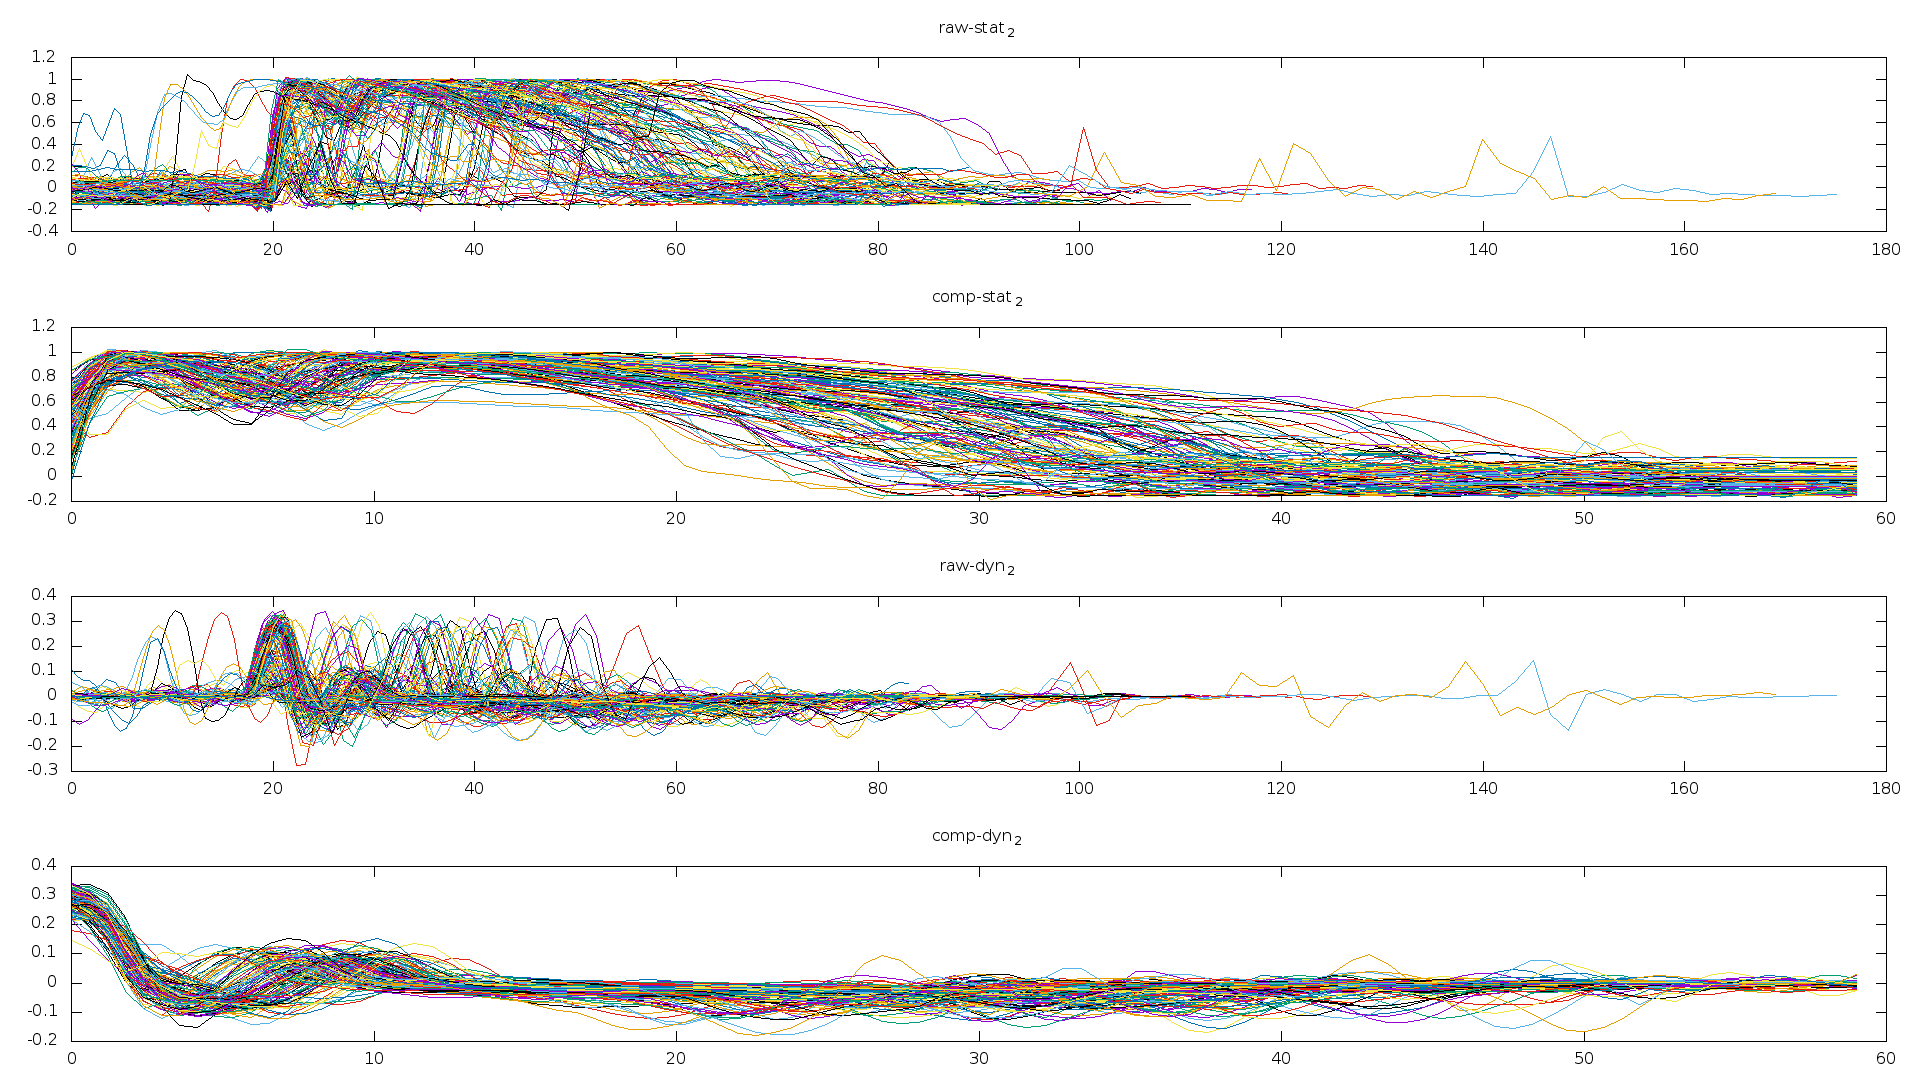
\includegraphics[scale=.3]{img/preprocessing.png}
	\caption{Repr\'esentation des \'en\'ergies statiques et dynamiques avant et
	apr\`es le traitement}
\end{figure}

Pour extraire les informations de la base de donn\'ee {\em TiDigits}, nous avons
utilis\'e le code que nous avions d\'evelopp\'e pour la premi\`ere partie du laboratoire.
Nous nous sommes bas\'es sur les similarit\'es entre la prononciation d'un
m\^eme chiffre par plusieurs individus. Pour cela, nous avons filtr\'e
les \'energies statiques et dynamiques afin de pouvoir accentuer les
propri\'et\'es de chaque chiffre.


Le filtrage consiste dans un premier temps \`a utiliser une op\'eration de
seuillage sur l'\'energie statique afin de d'\'et\'ecter le d\'ebut du mot et
d'\'eliminer tout le {\em blanc} qui se trouve au d\'ebut de l'enregistrement.
La seconde \'etape permet d'aligner le d\'ebut de chaque mot en utilisant le
premier maximum de l'\'energie dynamique.
Ceci nous permet de ne pas \^etre trop sensible aux diff\'erences d'attaque
entre les individus.

Comme tous les fichiers n'ont pas la m\^eme taille, nous devons ajouter
du padding afin que les donn\'ees puissent \^etre utilis\'ees comme
entr\'ee pour le r\'eseau. En effet, dans le cas o\`u les longueurs ne sont pas
identiques, il est impossible d'alimenter le r\'eseau en raison d'erreurs
de dimensions sur les produits matriciels.
D'autre part, dans le but d'am\'eliorer la vitesse de convergence de
l'apprentissage et de limiter la complexit\'e du mod\`ele, nous avons choisi de
ne garder que les donn\'ees statiques et de les normaliser, selon chaque colonne.
La figure \ref{fig:w_prep} donne un aper\c cu de l'impacte du pr\'e-traitement
sur les performances du r\'eseau.

La fonction d'extraction des donn\'ees {\em extract\_datasets()}
est con\c{c}ue pour prendre 2 param\`etres: le nombre de features d\'esir\'e
(40, 50, 60, ...) et un bool\'een permettant de choisir si l'on desir ou non
classifier selon le sexe de l'interpr\`ete. cette fonction retourne 3 listes:
un {\em training\_set}, un {\em validation\_set} et un {\em test\_set} o\`u
chaque \'el\'ement est une combinaison de 2 vecteurs les features {\bf x} et les
labels {\bf y}.

\lstset{tabsize = 4,
frame=lines,
numbers=left,
captionpos=b,
caption = {Fonction appele\'e pour extraire les donn\'ees d'un unique fichier},
language = python,
basicstyle=\small}
\begin{lstlisting}
def extract_sample(file_, size=60, sex=False, out_size=9):
    # Preprocess file ...
    x = prep.Preprocessing(file_, size)
    x.start_point_detection(threshold=0.5, n=10)
    x.cut_first_max(n=20)
    x.normalize()
    x.fit()
    x.get_subset('static')

    num = int(re.search(r'(?=.*)[0-9](?=.*)', file_).group(0))

    # make a column of the whole array
    features = x.data.reshape((len(x.data)*len(x.data[0]), 1) )

    if sex:
        if re.search(r'.*woman.*', file_):
            labels = vectorize_output( num - 1 + out_size, shape=(out_size*2, 1))
        else:
            labels = vectorize_output(num-1, shape=(out_size*2, 1))
    else:
        labels = vectorize_output(num-1, shape=(out_size, 1))

    return (features, labels)

\end{lstlisting}

\subsection{Initialisation du r\'eseau}
Lorsque le r\'eseau est instanci\'e, nous passons le nombre de centroide que nous voulons par classe.
Ensuite nous avons le choix entre 2 types d'initialisation.\\
Le premier choix permet d'initialiser avec des poids al\'etoire du dataset.

\lstset{tabsize = 4,
frame=lines,
numbers=left,
captionpos=b,
caption = {Initialisation des poids avec la m\'ethode},
language = python,
basicstyle=\small}
\begin{lstlisting}
def random_weight_init(input_size, output_size, ppc, tr_d):
    """ select codebooks at random within the dataset """

    weights = [ np.zeros(shape=(input_size, 1)) ] * (output_size * ppc)

    np.random.shuffle(tr_d)
    tr_dX = []
    tr_dY = []
    for x, y in tr_d:
        tr_dX.append(x)
        tr_dY.append(y)

    tr_dX = np.array(tr_dX)
    tr_dY = np.array(tr_dY)

    for w_idx, w in enumerate(weights):
        match = np.where(tr_dY == w_idx%output_size)[0][0]
        weights[w_idx] = tr_dX[match]

    return weights
\end{lstlisting}

\lstset{tabsize = 4,
frame=lines,
numbers=left,
captionpos=b,
caption = {Initialisation des poids avec la m\'ethode },
language = python,
basicstyle=\small}
\begin{lstlisting}
def average_weight_init(input_size, output_size, ppc, tr_d):
    """ init codebooks using the mean point """

    weights = [ np.zeros(shape=(input_size, 1)) ] * (output_size * ppc)

    np.random.shuffle(tr_d)
    tr_dX = []
    tr_dY = []
    for x, y in tr_d:
        tr_dX.append(x)
        tr_dY.append(y)

    tr_dX = np.array(tr_dX)
    tr_dY = np.array(tr_dY)

    for w_idx, w in enumerate(weights):
        match = np.where(tr_dY == w_idx%output_size)
        weights[w_idx] = np.mean(tr_dX[match], axis=0)

    return weights
\end{lstlisting}
\newpage



\paragraph{Validation crois\'ee:} Pour d\'etecter le sur-ajustement, il est
important de s\'eparer le set de donn\'ees en deux une partie pour l'entrainement
l'autre pour la validation. Plusieurs m\'ethodes diff\'erentes sont disponibles
pour d\'eterminer comment s\'eparer le dataset. Plus on \`a de donn\'ees dans le set
d'entrainement plus la pr\'ediction sera bonne mais moins on sera capable de
quantifier la capacit\'e de g\'en\'eralisation du r\'eseau et inversement.

Une m\'ethode int\'eressante \`a citer est le \href{http://work.caltech.edu/slides/slides13.pdf}
{\emph{V-folds} ou \emph{K-folds}} qui permet de maximiser le nombre d'\'echantillons
d'entrainement en divisant le set complet en $V$ sous ensembles. Le r\'eseau est
ensuite entrain\'e sur tous les sous-ensembles moins un qui est utilis\'e pour la
validation (le sous-ensemble de validation est choisi al\'eatoirement et change
\`a chaque \'epoque d'apprentissage). Il faut noter qu'il est important de
s\'electionner les \'echantillons de mani\`ere al\'eatoire afin de ne pas biaiser
l'apprentissage du r\'eseau.

Cependant, notre set de donn\'ees \'etant d\'ej\`a s\'epar\'e en plusieurs sous-ensembles,
nous garderons ces m\'ethodes comme pistes d'am\'elioration futures.

\paragraph{Detection: }Le sur-ajustement peut etre aisement d\'etect\'e lorsque
l'erreur sur le set de validation commence \`a augmenter tandis que l'erreur sur
le set d'entrainement continue de d\'ecroitre.

\paragraph{Early stopping} est une m\'ethode de limitation du sur-ajustement. Elle
consiste \`a monitorer les erreurs au cours de l'entrainement du r\'eseau et
de l'interrompre sous certaines conditions(seuil, moyenne glissante, ...).

\newpage
\subsection{Entrainement}
Lors de l'entrainement on passe comme param\`etre le nombre d'epochs, le taux d'apprentissage $\eta$ et $\eta_{decay}$ (diminution lin\'eaire du taux d'apprentissage).
L'entrainement du r\'eseau est un processus gourmand en calculs et demandant
beaucoup de ressources. Il est donc important de bien l'optimiser. Dans ce but,
nous sommes pass\'es par plusieurs m\'ethodes avant d'arriver \`a la plus optimale. C'est a dire de faire un choix qui avec un 



\lstset{tabsize = 4,
frame=lines,
numbers=left,
captionpos=b,
caption = {division du set ${\bf x}$ en sous-ensembles de taille $N$},
language = python,
basicstyle=\small}
\begin{lstlisting}
def train(self, tr_d, eta, epochs, eta_decay=False, va_d=None, estop=True):
	
	va_err, tr_err = [], []
	for i in xrange(0, epochs):
		for x, y in tr_d:
		    d = []
		    for w in self.weights:
		        # Compute distances
		        d.append(self.distance(x, w))

		    # find closest centroid
		    bmu = np.argmin(d)
		    # Update closest weight: Best Matching Unit
		    if bmu % self.output_size == y: 
		    	s = 1
		    else: 
		    	s = -1
		    self.weights[bmu] += s * eta * (x - self.weights[bmu])
		    
		if eta_decay:
            # Compute optimized learning rate
            eta = eta / (1 + s * eta) if eta < 1 else 1
            
        tr_err.append(self.eval_error_rate(tr_d))
        # Validation
        if va_d:
            va_err.append(self.eval_error_rate(va_d))
            # Stop early if validation error is very low
            if estop and va_err[-1] < 0.01: break

        self.learn_time = datetime.datetime.now() - self.learn_time
        
        return tr_err, va_err
\end{lstlisting}

\newpage
\subsection{Ajustement des hyper-param\`etres}
% http://neuralnetworksanddeeplearning.com/chap3.html#how_to_choose_a_neural_network's_hyper-parameters
\begin{table}[h]
	\centering
	\begin{tabular}{|c|c|c|c|c|c|c|c|c|c|c|c|c|c|}
		\hline
		dataset & out  & $\eta$ & $\eta_{decay}$ & epoch  & proto  & tr(\%) & va(\%) & test(\%) & t(s)\\
		\hline		
		40	& 18 & 0.1 & True & 6 & 10 & 3.4 & 0.9 & 9.9 & 20\\
		\hline
		\rowcolor{green}		
		40	& 18 & 0.5 & True & 10 & 10 & 2.8 & 5.5 & 8.4 & 29\\
		\hline		
		40	& 18 & 0.6 & True & 10 & 10 & 3.6 & 3.7 & 9.7 & 29\\
		\hline		
		40	& 18 & 0.5 & True & 20 & 20 & 1.7 & 6.5 & 8.8 & 112\\
		\hline		
		40	& 18 & 0.1 & True & 20 & 20 & 2.9 & 2.7 & 10.2 & 112\\
		\hline		
		40	& 18 & 0.01 & True & 20 & 20 & 6.6 & 3.7 & 12.7 & 121\\
		\hline		
		40	& 18 & 0.1 & False & 20 & 20 & 4.8 & 0.9 & 10.7 & 121\\
		\hline		
		40	& 9 & 0.1 & True & 1 & 20 & 4.0 & 0 & 5.7 & 3\\
		\hline		
		40	& 9 & 0.5 & True & 2 & 20 & 2.2 & 0 & 4.3 & 6\\
		\hline
		40	& 9 & 0.6 & True & 2 & 20 & 2.3 & 0 & 4.3 & 6\\
		\hline
		\rowcolor{green}
		40	& 9 & 0.5 & True & 2 & 21 & 2.4 & 0.9 & 3.2 & 7\\
		\hline
		50  & 9 & 0.5 & True & 2 & 21 & 2.4 & 0.9 & 3.2 & 7\\
		\hline
		60  & 9 & 0.5 & True & 20 & 21 & 2.4 & 0.9 & 3.2 & 38\\
		\hline
\end{tabular}
  \caption{Tableau r\'ecapitalif des tests effectu\'es sur les
	hyper-param\`etres sur un {\em i5 dual-core, 2.2GHz} pour le LVQ }
\end{table}


Pour obtenir la meilleur solution nous avons chercher en premier le
taux d'apprentissage $\eta$  qui donnait la plus petite erreur sur le training set,
ensuite nous avons ajust\'e le nombre de prototype r\'eseau avec et sans la r\'eduction du taux d'apprentissage. Nous pouvons conclure qu'aux vues des r\'esultats la meilleur configuration est pour un dataset de 40 \'echantillons avec un taux d'apprentissage de 0,5. Lorsque nous avons fait la classification homme/femme nous avons observ\'e qu\'a partir de 10 prototypes les performances sur le taux d'erreur du data test n'\'etaient pas am\'elior\'ees. En ce qui concerne la classification des chiffres uniquement le choix  du nombre de prototypes est le meilleur entre 21 et 22, avant ou apr\`es les valeurs les performances se d\'egradent.       
\newpage
\subsection{Comparaison avec le MLP}
\begin{table}[h]
	\centering
	\begin{tabular}{|c|c|c|c|c|c|c|c|c|c|c|c|c|c|}
		\hline
		dataset & out & $\sigma$  & cost & $\Omega$ & $\eta$ & $\lambda$ &
			epoch  & batch & hidden & tr(\%) & va(\%) & test(\%) & t(s)\\
		\hline		
		40	& 18 & s & C & L2 & 0.5 & 0.001 & 30 & 10 & 0 & 0 & 2 & 14 & 20 \\
		\hline
		40	& 9 & s & C & L2 & 0.5 & 0.001 & 30 & 10 & 0 & 1 & 1 & 7 & 20 \\
		\hline
\end{tabular}
  \caption{Tableau r\'ecapitalif des tests effectu\'es sur les
	hyper-param\`etres sur un {\em i5 dual-core, 2.2GHz} pour le MLP }
\end{table}
% http://neuralnetworksanddeeplearning.com/chap3.html#how_to_choose_a_neural_network's_hyper-parameters
\begin{table}[h]
	\centering
	\begin{tabular}{|c|c|c|c|c|c|c|c|c|c|c|c|c|c|}
		\hline
		dataset & out  & $\eta$ & $\eta_{decay}$ & epoch  & proto  & tr(\%) & va(\%) & test(\%) & t(s)\\
		\hline		
		40	& 18 & 0.5 & True & 10 & 10 & 2.8 & 5.5 & 8.4 & 29\\
		\hline
		40	& 9 & 0.5 & True & 2 & 21 & 2.4 & 0.9 & 3.2 & 7\\
		\hline
\end{tabular}
  \caption{Tableau r\'ecapitalif des tests effectu\'es sur les
	hyper-param\`etres sur un {\em i5 dual-core, 2.2GHz} pour le LVQ }
\end{table}


\newpage
\subsection{Inspection du res\'eau}
Parmis les contraintes obligatoires, il nous est aussi demand\'e de pouvoir
inspecter les couches cach\'ees du r\'eseau. Pour ce faire, nous tirons parti du
fait que {\em Python} est un language interpr\'et\'e et qu'il fournit \`a
l'utilisateur une interface int\'eractive(voir annexe \ref{inspect}).

En combinaison avec la possibilit\'e de savegarder l'\'etat des
objects {\em Network} sous la forme de fichiers (compress\'es ou non), nous
pouvons ais\'ement analyser chaque couche (voir annexe \ref{saveload}).

D'autre part, la conception du r\'eseau permetterai, avec peu d'effort, de coupler
plusieurs objects {\em Network} en un {\em super} r\'eseau.
Ceci pourrai \^etre fait en impl\'ementant les m\'ethodes {\em \_\_add\_\_()}
et {\em \_\_getslice\_\_()} pour respectivement concat\'ener et couper des objects
{\em Network}.

N'ayant pas eu besoin de ces op\'erations, ces m\'ethodes n'ont
cependant pas \'et\'e impl\'ement\'ees.





\section{Discussions}
\subsection{Problemes rencontr\'es}
Lors de l'entrainement du r\'eseau, nous avons d'abord \'et\'e confront\'e \`a
de tr\`es mauvaises performances. Nous avons initialement pens\'e que notre
pr\'e-traitement \'etait inefficace voir destructeur. En analysant les
performances plus en d\'etail,
nous nous sommes aper\c cu que le r\'eseau \'etait moins performant que si
nous lui faisions faire des pr\'edictions al\'eatoires
$\epsilon_{\bf x} \ge \left (1 - \frac{1}{9} = 88.9\% \right)$.
Ce qui est impossible et sugg\`ere que notre \'evaluation du co\^ut \'etait fausse.

En effet, nous avions commis une erreur dans la g\'en\'eration de nos vecteurs de
sortie. Lorsque la pr\'ediction \'etait compar\'ee \`a la sortie attendue,
celle-ci \'etait d\'ecal\'ee de 1 comme suit:
\begin{equation}
	\left (
	{\bf \hat y}_3 =
	\begin{bmatrix}
		0 \\
		0 \\
		{\color{red} 1 }\\
		0 \\
		0 \\
		0 \\
		0 \\
		0 \\
		0 \\
	\end{bmatrix}
	\right )
	\ne
	\left (
	{\bf y}_3 =
	\begin{bmatrix}
		0 \\
		0 \\
		0 \\
		{\color{red} 1 }\\
		0 \\
		0 \\
		0 \\
		0 \\
		0 \\
	\end{bmatrix}
	\right )
\end{equation}

\subsection{Conclusion et pistes d'am\'elioration}
Comme expliqu\'e pr\'ec\'edement, du \`a un manque de temps, nous avons
\'et\'e contrain de couper certaines optimisations notemment sur
l'impl\'ementation matricielle du {\em Mini-batch SGD}.

En revanche, malgr\'e cela, on observe tout de m\^eme de bonnes performances.
En utilisant comme r\'ef\'erence une classification de 9 digits en combinaison
avec une classification Homme/Femme (soit une sortie de 18 neurones) du
{\em TiDigits} dataset, on obtient un temps d'entrainement de 10 secondes sur un
{\em i5 dual-core, 2.2GHz} temps qui tombe \`a moins de 2 secondes sur un
{\em i7 quad-core, 4GHz}.

On remarque aussi une bonne capacit\'e de g\'en\'eralisation avec une erreur
d'environs 10-15\% sur le set de test apr\`es l'apprentissage.

En observant attentivement les matrices de
confusions en figure \ref{fig:w_prep} on remarque que le r\'eseau commet
principalement des erreurs lors de la classification Homme/Femme. Ceci pourrait
probablement \^etre du \`a un pr\'e-traitement trop {\em agressif} ou encore \`a
manque d'\'echantillons d'entrainement. Cette classification erron\'ee pourrait
peut-\^etre \^etre ajust\'ee en impl\'ementant une m\'ethode de
validation-crois\'ee plus avanc\'ee telle que le {\em V-folds} cit\'e pr\'ec\'edemment.

D'autres pistes d'am\'eliorations seraient d'ajouter la possibilit\'e de choisir une
fonctions d'activation diff\'erente pour la couche de sortie ou encore
l'impl\'ementation de techniques permettant de determiner {\em automatiquement}
les hyper-param\`eters du r\'eseau.


%\newpage
%\appendix
%\section{Influences du pr\'e-traitement sur les performances du r\'eseau}
%\begin{figure}[htp]
%    \centering
%    \subfloat{{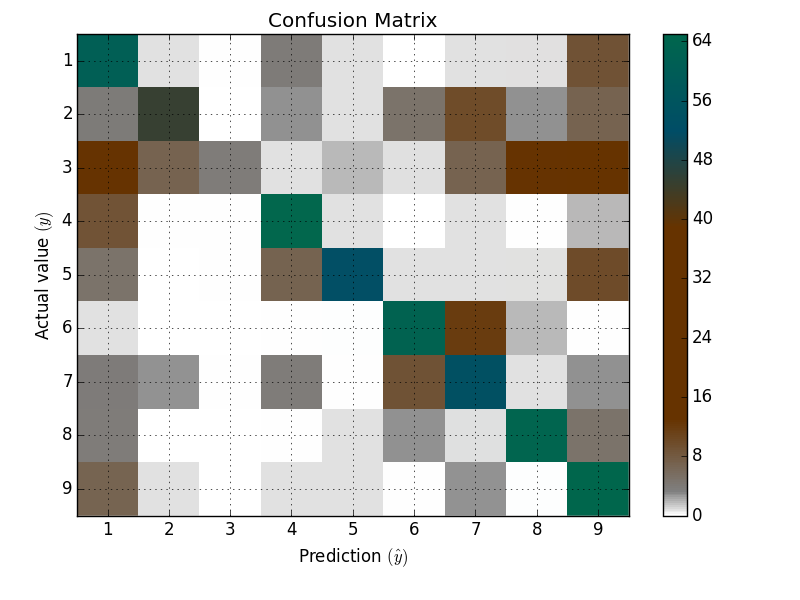
\includegraphics[width=.45\textwidth]{img/confusion_wo_prep.png} }}
%    \subfloat{{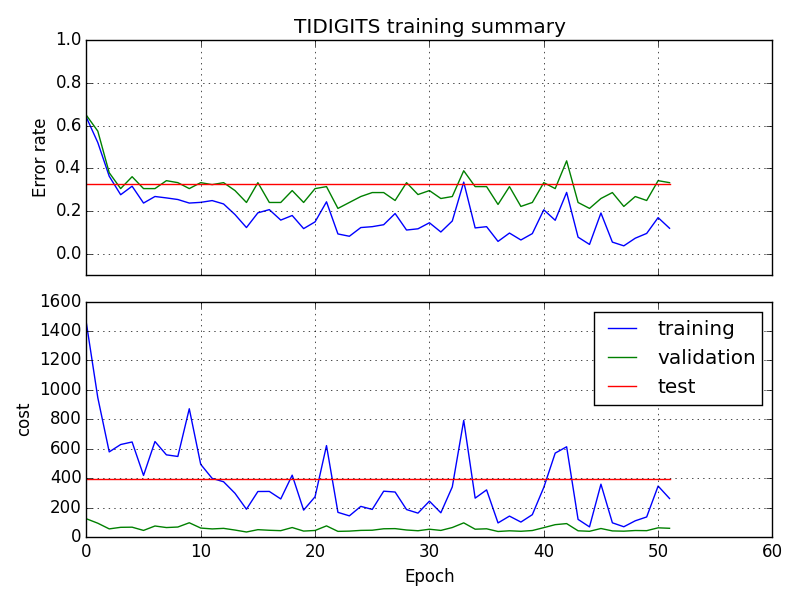
\includegraphics[width=.45\textwidth]{img/training_wo_prep.png} }}
%    \caption{Performances sans pr\'e-traitement}
%    \subfloat{{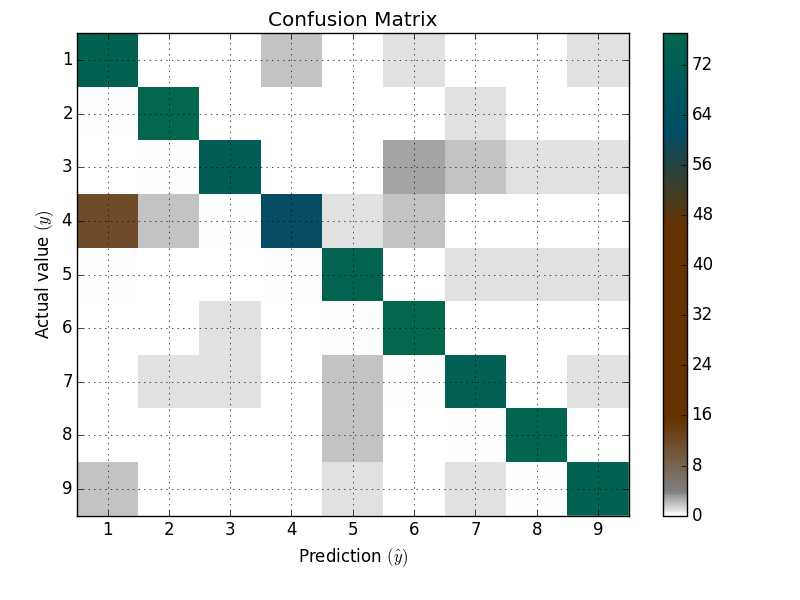
\includegraphics[width=.45\textwidth]{img/confusion_w_prep.png} }}
%    \subfloat{{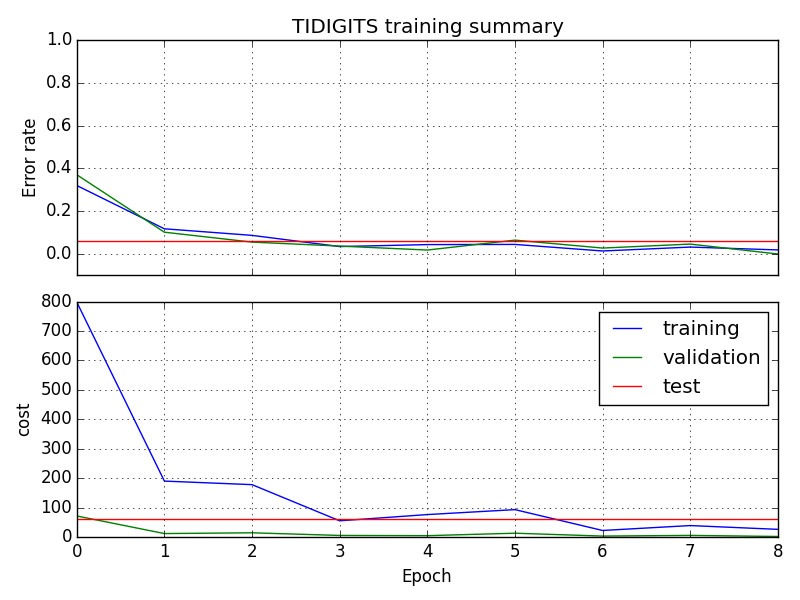
\includegraphics[width=.45\textwidth]{img/training_w_prep.png} }}
%    \caption{Performances avec pr\'e-traitement}
%    \label{fig:w_prep}
%\end{figure}
%\begin{figure}[htp]
%    \centering
%    \subfloat{{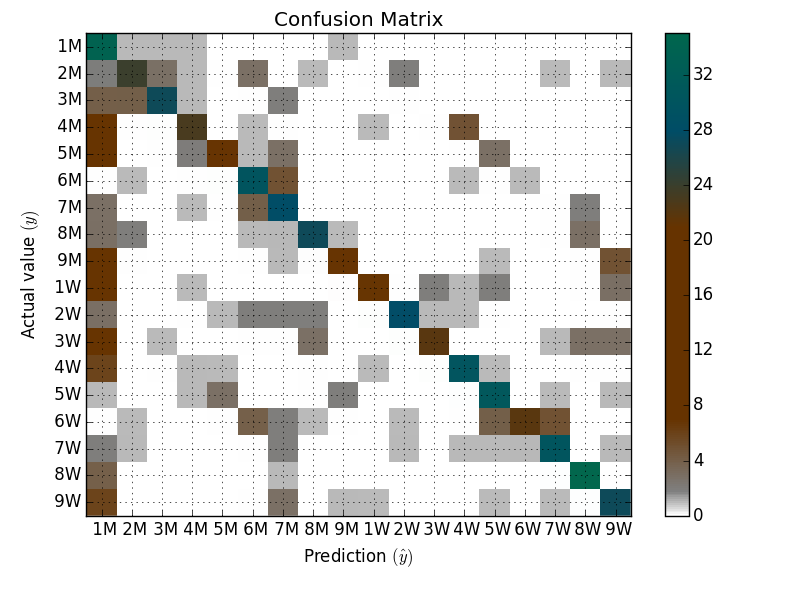
\includegraphics[width=.45\textwidth]{img/confusion_swo_prep.png} }}
%    \subfloat{{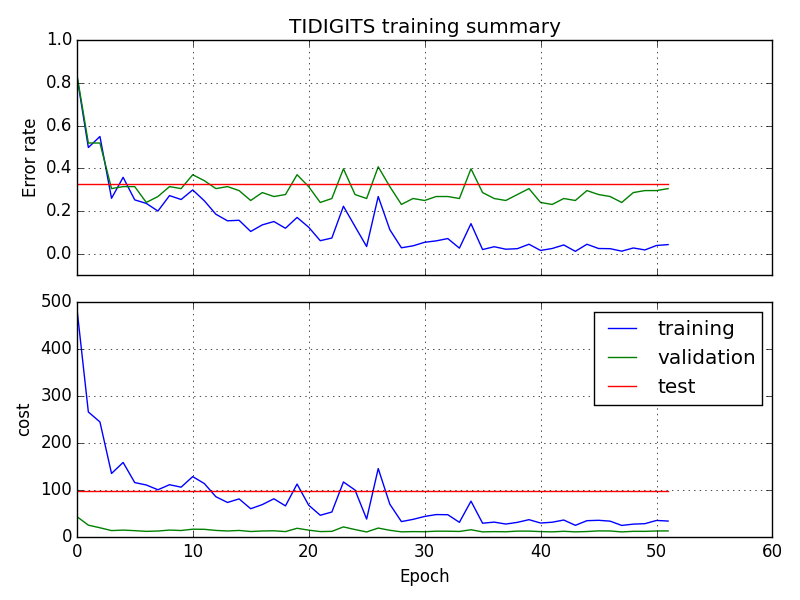
\includegraphics[width=.45\textwidth]{img/training_swo_prep.png} }}
%    \caption{Performances sans pr\'e-traitement}
%    \subfloat{{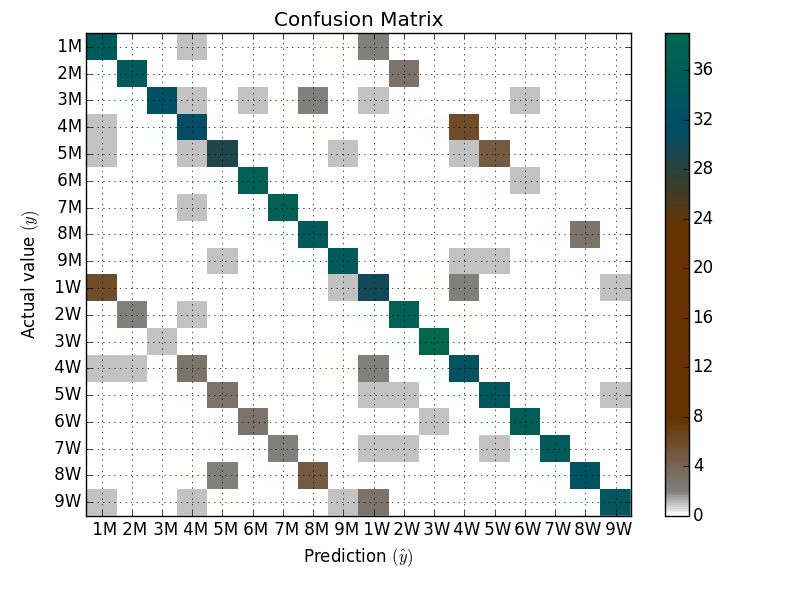
\includegraphics[width=.45\textwidth]{img/confusion_sw_prep.png} }}
%    \subfloat{{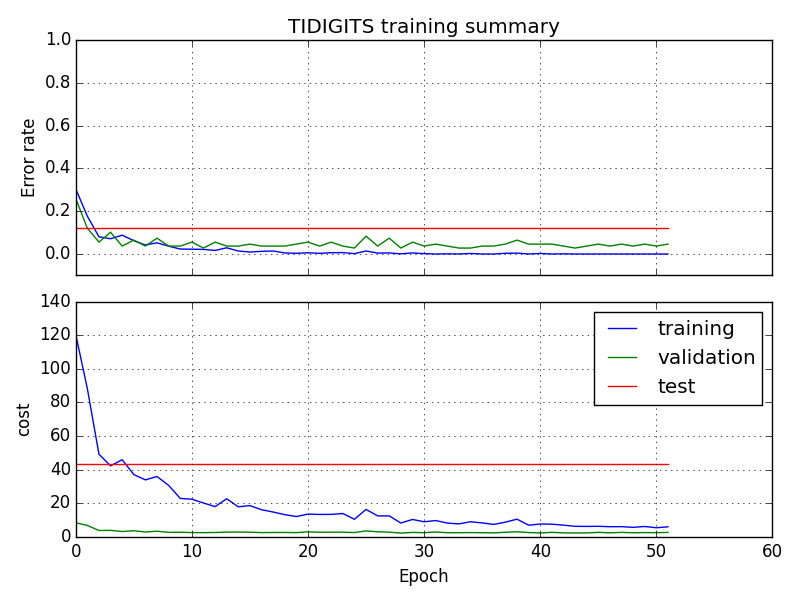
\includegraphics[width=.45\textwidth]{img/training_sw_prep.png} }}
%    \caption{Performances avec pr\'e-traitement}
%    \label{fig:w_prep}
%\end{figure}
%\newpage
%\section{sauvegarde/chargement d'une configuration}
%\label{saveload}
%\lstset{tabsize = 4,
%frame=lines,
%numbers=none,
%captionpos=b,
%caption = {Sauvegarde et chargement interactif d'une configuration},
%language = python,
%basicstyle=\small}
%\begin{lstlisting}
%In [1]: import network as n
%In [2]: my_net = n.Network([3, 4, 2], activation='sigmoid',
%                   cost='cross-entropy', learning_rate=0.5)
%In [3]: print my_net
%Neural Network      : [3, 4, 2]
%Activation function : sigmoid
%Cost function       : cross-entropy
%Regularization func : none
%learning rate       : 0.5
%Regularization rate : 0.1
%
%L0  * * *
%L1 * * * *
%L2   * *
%In [4]: my_net.save('foo.save')
%In [5]: my_net = n.Network([8, 4, 4, 2], activation='tanh',
%   ...:                   cost='quadratic', learning_rate=0.02,
%   ...:				      regularization='L2', lambda_ = 0.001)
%In [6]: print my_net
%Neural Network      : [8, 4, 4, 2]
%Activation function : tanh
%Cost function       : quadratic
%Regularization func : L2
%learning rate       : 0.02
%Regularization rate : 0.001
%
%L0 * * * * * * * *
%L1     * * * *
%L2     * * * *
%L3       * *
%In [7]: my_net.load('foo.save')
%In [8]: print my_net
%Neural Network      : [3, 4, 2]
%Activation function : sigmoid
%Cost function       : cross-entropy
%Regularization func : none
%learning rate       : 0.5
%Regularization rate : 0.1
%
%L0  * * *
%L1 * * * *
%L2   * *
%\end{lstlisting}
%
%\newpage
%\section{Inspection du r\'eseau}
%\label{inspect}
%\lstset{tabsize = 4,
%frame=lines,
%numbers=none,
%captionpos=b,
%caption = {Exemple d'inspection interactive d'un r\'eseau de neurones},
%language = python,
%basicstyle=\small}
%\begin{lstlisting}
%In [1]: import network as n
%In [2]: my_net = n.Network((1, 2))
%In [3]: my_net.load('foo.save')
%In [4]: print my_net.struct
%[3, 4, 2]
%
%In [15]: print my_net.weights[0]
%[[ 0.12737432  0.97734051 -0.56505148]
% [ 0.9090921   0.19178132 -0.15200818]
% [-0.07138651 -0.59903432 -0.78958921]
% [-0.55362229  0.51319807  0.2935551 ]]
%
%In [16]: print my_net.weights[1]
%[[-0.69519106  0.15539354 -0.46978019 -0.88703575]
% [-0.44994898 -0.57113777 -0.3736959  -0.00245537]]
%
%In [17]: cat foo.save
%# vim: set ft=yaml:
%activation: sigmoid
%biases:
%- - [-0.920441751728251]
%  - [-0.36244765002601287]
%  - [-0.2926753984327689]
%  - [-0.12034180777419923]
%- - [1.1212748305651405]
%  - [-0.565286303186786]
%cost: cross-entropy
%eta: 0.5
%lambda: 0.1
%regularization: none
%struct: [3, 4, 2]
%weights:
%- - [0.12737431801447707, 0.9773405101355827, -0.5650514778232817]
%  - [0.90909209744093, 0.19178132268834805, -0.1520081800115934]
%  - [-0.07138650509286246, -0.5990343151487274, -0.7895892103519402]
%  - [-0.5536222909987745, 0.5131980654305697, 0.29355509901743354]
%- - [-0.6951910582048451, 0.1553935350379862, -0.4697801922017521,
%		-0.8870357534796379]
%  - [-0.44994897980803156, -0.5711377657299319, -0.3736959026341852,
%		-0.002455368584577519]
%\end{lstlisting}
%
%\section{Visuels de l'interface graphique} \label{gui}
%\begin{figure}[htp]
%	\centering
%	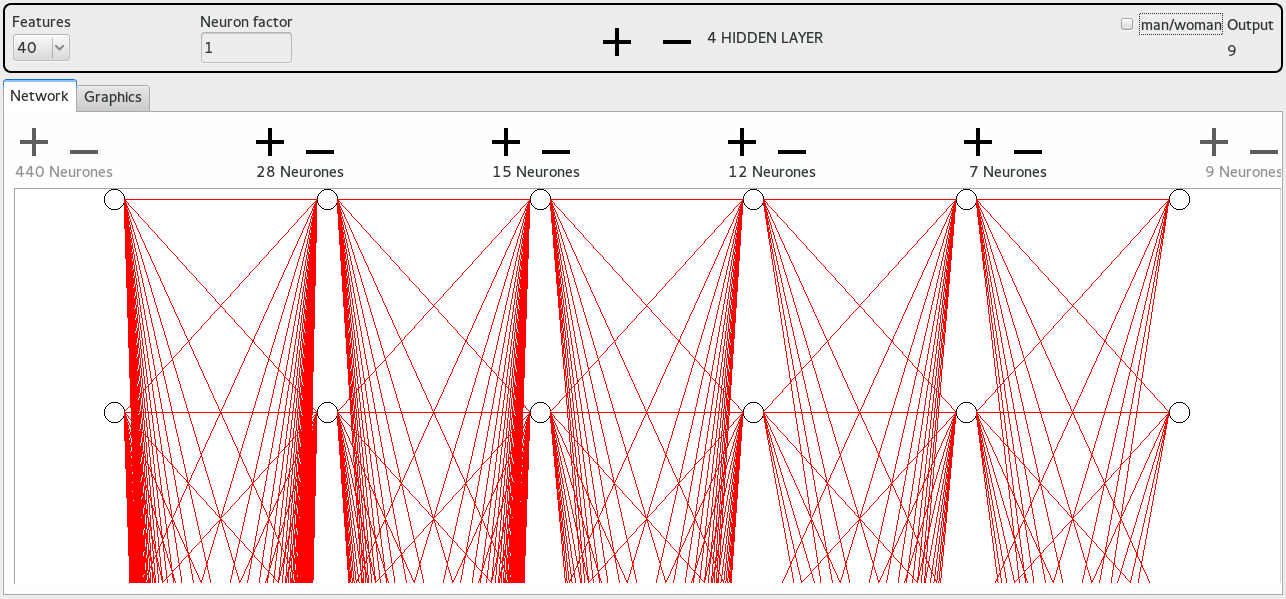
\includegraphics[scale=.27]{img/NetworkGraphics.png}
%	\caption{Repr\'esentation visuelle du r\'eseau}
%	\label{guinet}
%\end{figure}
%
%\begin{figure}[htp]
%	\centering
%	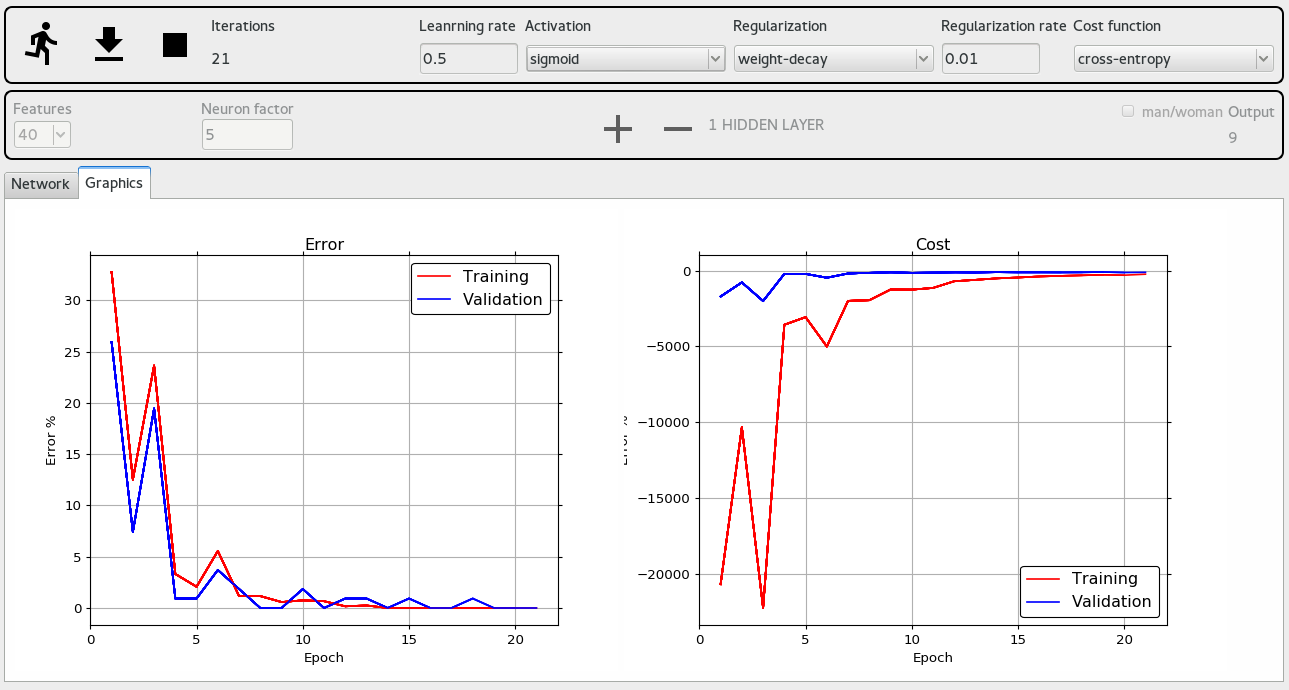
\includegraphics[scale=.27]{img/courbe.png}
%	\caption{Affichage des courbes d'erreur et de co\^ut}
%	\label{guierr}
%\end{figure}
%
%
\end{document}
% vim: cc=80 :
